% Lab 10 on Recursion
%
% CSE/IT 107: Introduction to Programming
% New Mexico Tech
%
\documentclass[11pt]{cselabheader}

%%%%%%%%%%%%%%%%%% SET TITLES %%%%%%%%%%%%%%%%%%%%%%%%%
\fancyhead[R]{Lab 10: Recursion}
\title{Lab 10: Recursion}

\begin{document}

\maketitle
\pagenumbering{roman}
\hrule

\begin{quote}
``A mirror mirroring a mirror.''

``In the end, we self-perceiving, self-inventing, locked-in mirages
are little miracles of self-reference.''
\end{quote}
\begin{flushright}
--- Douglas R. Hofstadter, I Am a Strange Loop
\end{flushright}

\hrule

\begin{figure}[H]
  \centering
  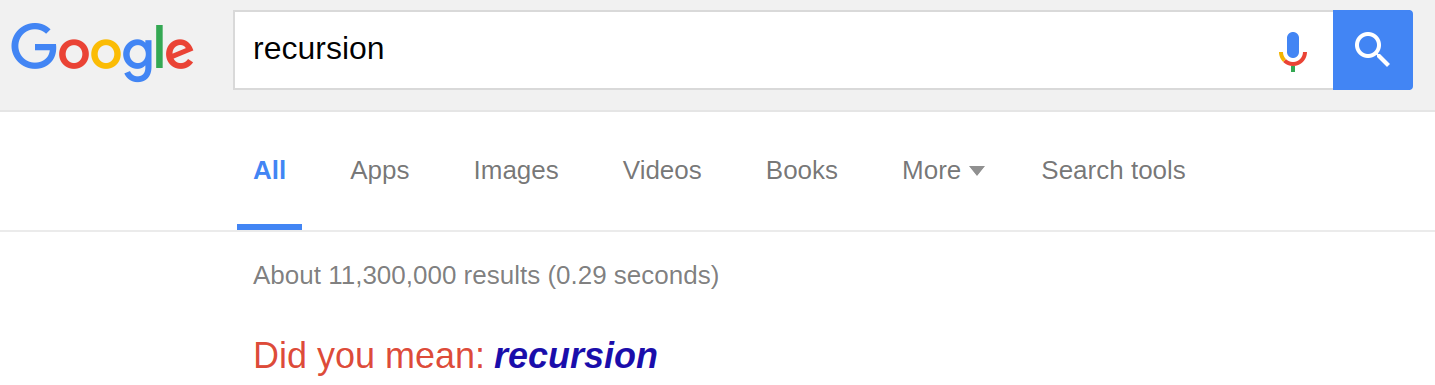
\includegraphics[width=\textwidth]{img/didyoumean.png}
  \caption{Google search for recursion (2016).}
\end{figure}

\begin{figure}[H]
  \centering
  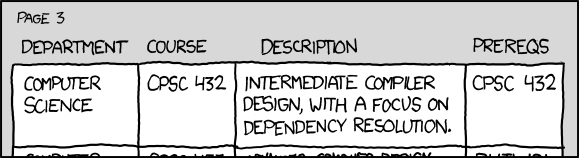
\includegraphics[width=0.5\textwidth]{img/xkcd_dependencies.png}
  \caption{Dependencies \url{http://xkcd.com/754/}}
\end{figure}

\hrule

\pagebreak
\section*{Introduction}
\addcontentsline{toc}{section}{Introduction}

You have learned about while loops, Python lists and how to manipulate
the elements in a list using for-loops and list comprehensions.  In
this lab you will learn about recursion.  Recursion can be used to
iterate through complicated data structures and to replicate the
functionality offered by while loops and for loops.  We will look at
some examples of recursive functions and the type of problems
recursion can help solve.

\tableofcontents

\pagebreak
\pagenumbering{arabic}

\section{A Simple Recursive Function}

How does Python evaluate this function?

\begin{python3code}
def count(n):
    print(n)
    count(n + 1)
count(0)
\end{python3code}

This function never stops running. It is similar to the following while loop.

\begin{python3code}
n = 0
while True:
    print(n)
    n += 1
\end{python3code}

Line 3 of the \pythoninline{count()} function is an example of a
recursive call.  This means that within the function body the function
calls itself. In this lab, we will explore these \textsl{recursive functions}.

\section{Termination}

How do you make a recursive function stop running?  Don't allow it to
call itself every time. For example, this function only calls itself
when its argument \inlinepython{problems} is greater than 1.

\begin{python3code}
def how_to_do_homework(problems):
    print("How to do {} homework problems".format(problems))
    if problems <= 1:
        print("Do the problem and then you're done.")
    else:
        print("Do the first problem and then do {} problems".format(problems))
        problems -= 1  # get rid of one problem
        how_to_do_homework(problems) # then do the rest of the problems
\end{python3code}

If we call the function with the argument \pythoninline{problems} set to 5,
Python will print this output:

\begin{verbatimcode}
How do you do 5 homework problems?
Do the first one and then do 4 problems.
How do you do 4 homework problems?
Do the first one and then do 3 problems.
How do you do 3 homework problems?
Do the first one and then do 2 problems.
How do you do 2 homework problems?
Do the first one and then do 1 problems.
How do you do 1 homework problems?
Do the problem and then you're done.
\end{verbatimcode}

\section{Examples with One Recursive Call}
\subsection{Iterating through Lists}

Here is an example function that adds 1 to every element in a list.
First, the function checks if the list is non-empty. If so, it adds
one to the first element and appends that element to the rest of
the list. The rest of the list is passed as an argument to the
recursive call.

This code is an \textsl{unrealistic} way of traversing a list. It
would be better to use a list comprehension or a for-loop.

\begin{python3code}
def add(elements):
    if len(elements) == 0:
        return []
    first_element = elements[0] + 1  # add 1 to the first element
    rest_of_list = elements[1:]  # shrink the list

    # work on the rest of the list
    return [first_element] + add(rest_of_list)
\end{python3code}

What happens when we call this function? Here is a step-by-step
example of running \pythoninline{add([1,2,3])}.

\begin{description}
\item[Input of the first function call:] \pythoninline{[1, 2, 3]}

First the function checks if the list is non-empty, then it adds 1 the
first element and calls itself with a shorter input.

\item[Input of recursive call 1:] \pythoninline{[2, 3]}

This next function call also checks that the list is non-empty, it adds 1
to the first element and calls itself with an even shorter list.

\item[Input of recursive call 2:] \pythoninline{[3]}

Same thing happens with this input.

\item[Input of recursive call 3:] \pythoninline{[]}

There are no elements to add 1 to.

\item[Output of recursive call 3:] \pythoninline{[]}

When this function receives the empty list, it returns an empty list.

\item[Output of recursive call 2:] \pythoninline{[3 + 1] + []}

Function call 3 gets a list and adds an element to it.

\item[Output of recursive call 1:] \pythoninline{[2 + 1] + [3 + 1] + []}

Function call 2 also gets a list and adds an element to it.

\item[Output of the first function call:] \pythoninline{[3 + 1] + [2 + 1] + [3 + 1] + [] = [4, 3, 2]}

Finally, function call 1 gets the last two elements, adds the very
first element after adding 1 and then returns final result.
\end{description}

When a function makes a recursive call by calling itself with a smaller input,
it is requesting that the same thing be done to that smaller input.
In this case, the first function call to \pythoninline{add} added 1 to the
first value of the list and then passed off the rest of the work to
function call 2. Function call 2 added 1 to the second element of the list,
and passed the rest of the work on to function call 3. This happened until
there were no more numbers in the list.

\subsection{Recursion in Mathematics}
Recursive calls are not just for iterating through data, they can also be used
for computations of arbitrary length. A common example of a recursive function
is the factorial. The factorial of a number is the product of all numbers from
1 to that number, for example
\begin{align*}
\text{factorial of } 1 &= 1
\\
\text{factorial of } 2 &= 1 \cdot 2 = 2
\\
\text{factorial of } 3 &= 1 \cdot 2 \cdot 3 = 6
\\
\text{factorial of } 4 &= 1 \cdot 2 \cdot 3 \cdot 4 = 24
\\
\text{factorial of } 50 &= 1 \cdot 2 \cdot 3 \cdot 4 \cdot 5
                         \dotsb \cdot 49 \cdot 50
\\ &= 30414093201713378043612608166064768844377641568960512000000000000
\end{align*}

The code is very close to a mathematical definition of the factorial:

\begin{python3code}
def factorial(n):
    if n <= 1:
        return 1
    return n * factorial(n - 1)
\end{python3code}

In order to compute the factorial of an integer, you must compute the
factorial of a smaller integer. Some examples. Note, unlike many other programming languages Python
supports huge integers.

\begin{pyconcode}
>>> factorial(1)
1
>>> factorial(4)
24
>>> factorial(50)
30414093201713378043612608166064768844377641568960512000000000000
\end{pyconcode}

\section{Examples with Multiple Recursive Calls}
\subsection{Iterating through Nested Lists}

Recursion is especially useful when dealing with deeply nested data structures.
These include trees, graphs, and other data structures that are introduced in
higher level CS classes. We will focus on nested lists. Consider this list:

\begin{python3code}
[1, 2, [3, 4, [5, 6]], [7]]
\end{python3code}

What if we want to add 1 to every number in this list?

A useful code fragment when dealing with such a list is
\pythoninline{type(element) == list}.  This checks if the value of
\pythoninline{element} is a Python list.  We can use it to decide
whether to add 1 to an element of a nested list or to add 1 to all of
its sub-elements.

\begin{python3code}
def add1(nested_list):
    new_list = []
    for element in nested_list:
        if type(element) == list:
            # if the element is a list
            # add 1 to each of its elements
            new_list.append(add1(element))
        else:
            # otherwise, just add 1 to the element
            new_list.append(element + 1)
    return new_list
\end{python3code}

We get these results:

\begin{python3code}
>>> add1([1, 2, 3])
[2, 3, 4]
>>> add1([1, 2, [3, 4, [5, 6]], [7]])
[2, 3, [4, 5, [6, 7]], [8]]
\end{python3code}

Here a description of what the function \pythoninline{add1} did in the
second example.

\begin{enumerate}
\item The function starts iterating through the given list.
\item \pythoninline{element = 1}

The first element is an integer, so

\pythoninline{new_list = [1 + 1]}

\item \pythoninline{element = 2}

\pythoninline{new_list = [2, 3]}

\item \pythoninline{element = [3, 4, [5]]}

We need to make a recursive call to add 1 to every element of this
sub-list. Essentially, the list looks like this now:

\pythoninline{new_list = [2, 3, add1([3, 4, [5]])]}

The recursive call to \pythoninline{add1} makes its own recursive call
in order to compute the last element of its return value:

\pythoninline{[4, 5, add1([5])]}.

The end result is \pythoninline{[4, 5, [6]]}.
So after two recursive calls, we have:

\pythoninline{new_list = [2, 3, [4, 5, [6]]]}

\item \pythoninline{element = [7]}

This is a list, so a recursive call is made. A for loop
iterates through the one-element list. In this recursive call
\pythoninline{element = 7}, so 8 is added to the new list and
the recursive call to the function returns \pythoninline{[8]}.

\pythoninline{new_list = [2, 3, [4, 5, [6]], [8]]}

\item \pythoninline{add1} has finished iterating through the list.
\end{enumerate}

We can also think of these recursion calls like this:

\begin{description}
\item[First function call] \pythoninline{add1([1, 2, [3, 4, [5, 6]], [7]])}
\item[Recursive call 1] \pythoninline{[2, 3, add1([3, 4, [5, 6]]), add1([7])]}
\item[Recursive call 2] \pythoninline{[2, 3, [4, 5, add1([5, 6])], [8]]}
\item[End result] \pythoninline{[2, 3, [4, 5, [6, 7]], [8]]}
\end{description}


Here is another function that works on nested lists.
It counts the number of integers or other ``non-lists'' in a nested list.
For example,

\begin{pyconcode}
>>> elements_in([])
0
>>> elements_in([[[[]]]])
0
>>> elements_in([100, 200])
2
>>> elements_in([1, 2, [3, 4, [5, 6]], [7]])
7
\end{pyconcode}

This is the code for this recursive function. Recursive calls are made to count
the number of elements in each sub-list. Try to run this code.

\begin{python3code}
def elements_in(nested_list):
    count = 0
    for element in nested_list:
        if type(element) == list:
            # count the number of elements in a sub-list
            count = elements_in(element)
        else:
            # otherwise, just add 1 to the count
            count += 1
    return count
\end{python3code}

\subsection{Drawing A Tree}

We can have multiple recursive calls in a function. To draw a type of tree,
we can use the turtle module to do the following:

\begin{enumerate}
\item If enough has been drawn, stop.
\item Otherwise, draw a straight line.
\item Save position and heading (the direction of the turtle)
\item \textbf{(Recursive call)} Draw a tree half as big as this one
and place it towards the right.
\item When finished drawing that tree, restore position and heading.
\item \textbf{(Recursive call)} Do the same thing to draw a tree to
the left.
\item Finished.
\end{enumerate}

In code, this looks like:

\begin{python3code}
import turtle

def draw_tree(branch_size, max_branches=5):
    # done drawing?
    if max_branches <= 0:
        return

    turtle.speed("fastest")

    # start drawing
    turtle.pendown()
    turtle.forward(branch_size)
    # do not draw anything else
    turtle.penup()

    # save the current position and direction
    p, h = turtle.position(), turtle.heading()

    # draw the right branch
    turtle.right(45)
    draw_tree(branch_size / 2, max_branches - 1)

    # jump back
    turtle.setposition(p)
    turtle.setheading(h)

    # draw the left branch
    turtle.left(45)
    draw_tree(branch_size / 2, max_branches - 1)

def main():
    # face up
    turtle.left(90)
    draw_tree(200, max_branches=9)
    turtle.done()

if __name__ == "__main__":
    main()
\end{python3code}

Notice the instructions ask to draw a smaller tree while drawing a tree.
This self-referential instruction is translated into the recursive calls
on lines %%% LINES
This code generates this turtle graphic:

\begin{center}
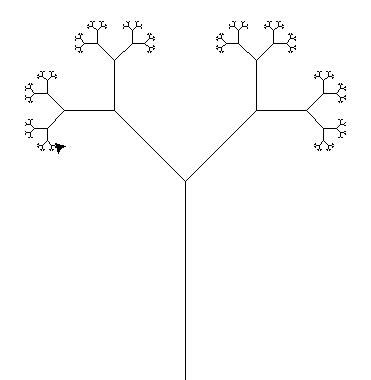
\includegraphics[width=0.5\linewidth]{img/tree.png}
\end{center}

\section{Overview}
\begin{itemize}
\item A typical recursive function calls itself one or more times.
\item A recursive function that finishes has a condition that causes
it to stop calling itself.
\item Whenever a problem needs small parts of its own solution in
order to be solved, a recursive function may make a good solution.
\end{itemize}

Recursion is useful when dealing with nested data structures. When
a problem can be solved by solving smaller versions of the problem, a
recursive function might make a good solution.  Recursion is used to
sort lists of data, to read and run computer programs, to solve
mathematical problems, and for many other problems. Anything you can
do with a while loop or a for loop can be done using a recursive function.

\newpage
\section{Exercises}

\begin{ex}[palindrome.py] Write a recursive function that determines whether a
    string is a palindrome. A palindrome is a word that is the same forwards and
    backwards, for example ``abba''.

    The function should take in only one argument (the string to check) and
    return either \lstinline{True} or \lstinline{False}.

    It is required that your function must be recursive and take only one argument.
    This is not the easiest way to check if a string is a palindrome, but the goal
    is to solve a problem recursively, not to check if a value is a palindrome.
\end{ex}

\begin{ex}[nested.py]
Write a function named \pythoninline{element_of} that returns
\pythoninline{True} if a given element is in a nested list and
\pythoninline{False} otherwise.

This function must have at least one recursive call.

\begin{pyconcode}
>>> import nested
>>> nested.element_of(5, [1,2,3,4,5,6,7])
True
>>> nested.element_of(7, [1,2,[3,4,[5,6]],[7]], 1)
True
>>> nested.element_of(77, [1,2,[3,4,[5,6]],[7]], 1)
False
\end{pyconcode}
\end{ex}

\begin{ex}[cesaro.py]
Write a recursive function that draws the Cesaro torn line fractal to
arbitrary depth. It is recommended to call
\pythoninline{turtle.speed('fastest')} in order to speed up drawing.

Here are the Cesaro torn line fractals at depths 1, 2, and 6.
\begin{center}
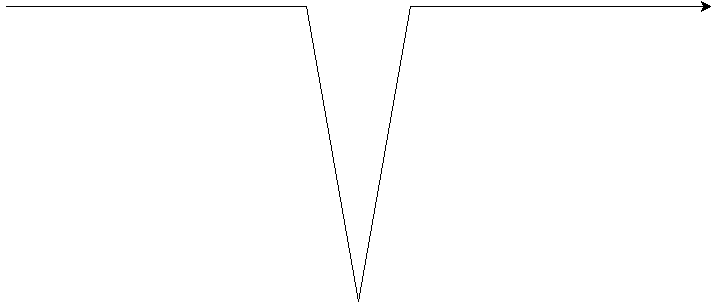
\includegraphics[width=0.4\textwidth]{img/cesaro1.png}
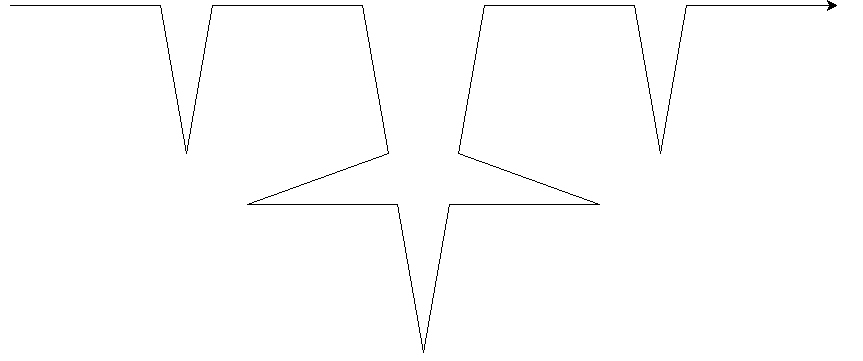
\includegraphics[width=0.4\textwidth]{img/cesaro2.png}
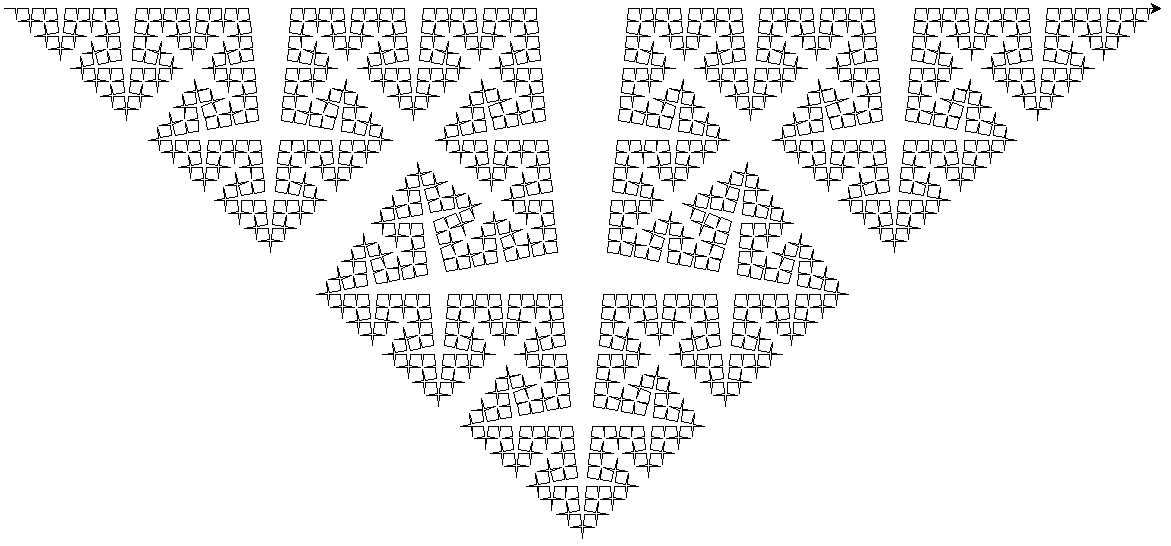
\includegraphics[width=0.8\textwidth]{img/cesaro6.png}

Turtle was not made for depth 9, but here it is:
\includegraphics[width=0.9\textwidth]{img/cesaro9.png}
\end{center}

Hints:
\begin{itemize}
\item Using the Turtle module, the depth 0 Cesaro fractal of a width
\pythoninline{w} is just \pythoninline{turtle.forward(w)}.
\item Start by drawing the Cesaro fractal at depth one. This should
not need any recursion.
\item Replace all calls to the \pythoninline{turtle.forward} function
with recursive calls to draw smaller Cesaro fractals of a lower depth.
\end{itemize}
\end{ex}

\newpage
\section{Submitting}

You should submit your code as a tarball. It should contain all files
used in the exercises for this lab. The submitted file should be named
\begin{center}
  \texttt{cse107\_firstname\_lastname\_lab10.tar.gz}
\end{center}

\begin{center}
  \textbf{Upload your tarball to Canvas.}
\end{center}

\listofexercises

\end{document}
